\chapter{插值法}

\section{引言}

\begin{definition}[插值法]
    设函数$y=f(x)$在区间$[a,b]$上有定义, 且已知在点$a\le x_0\le x_1<\cdots<x_n\le b$上的值$y_0,y_1,\cdots,y_n$, 若存在
    一简单函数$P(x)$, 使
    \begin{equation}\label{eqn:2.1.1}
        P(x_i) = y_i,i=0,1,\cdots,n
    \end{equation}
    成立, 则称$P(x)$为函数$f(x)$的\emph{插值函数}, 点$x_0,x_1,\cdots,x_n$为\emph{插值节点}, 包括插值节点的区间$[a,b]$称为
    \emph{插值区间}, 求插值函数$P(x)$的方法称为\emph{插值法}.
\end{definition}

\begin{definition}[多项式插值]
    若$P(x)$是次数不超过$n$的代数多项式, 即
    \begin{equation}\label{eqn:2.1.2}
        P(x) = a_0+a_1x+\cdots+a_nx^n
    \end{equation}
    其中$a_i$为实数, 则称$P(x)$为\emph{插值多项式}, 相应的插值法称为\emph{多项式插值}.
\end{definition}

本章所讨论的主要内容是\emph{多项式插值}.

在寻找插值多项式之前, 需要对其存在性与唯一性进行讨论\footnote{存在性表明插值多项式存在, 唯一性表明无论采用哪种插值方法,
得到的结果是唯一的.}. 给出如下定理:

\begin{theorem}
    对于给定互异节点$x_0,x_1,\cdots,x_n$, 满足插值条件式(\ref{eqn:2.1.1})的$n$阶插值多项式(\ref{eqn:2.1.2})存在且唯一.
\end{theorem}

\begin{proof}
    设所要构造的插值多项式为
    \begin{equation*}
        P_n(x)=a_0+a_1x+\cdots+a_nx^n
    \end{equation*}
    由插值条件
    \begin{equation*}
        P_n(x_i) = y_i, i=0,1,\cdots,n
    \end{equation*}
    得如下线性方程组
    \begin{equation*}
        \begin{cases}
            1\cdot a_0+x_0a_1+\cdots+x_0^na_n=y_0\\
            1\cdot a_0+x_1a_1+\cdots+x_1^na_n=y_1\\
            \vdots\\
            1\cdot a_0+x_na_1+\cdots+x_n^na_n=y_n
        \end{cases}
    \end{equation*}
    求解$a_0, a_1, \cdots, a_n$, 计算系数行列式
    \begin{equation*}
        D = \mqty|1&x_0&x_0^2&\cdots&x_0^n\\
        1&x_1&x_1^2&\cdots&x_1^n\\
        \vdots&\vdots&\vdots&&\vdots\\
        1&x_n&x_n^2&\cdots&x_n^n|
    \end{equation*}
    该行列式为Vandermonde行列式, 其值为
    \begin{equation*}
        D = \prod_{0\le j<i\le n}(x_i-x_j)
    \end{equation*}
    当$x_i\ne x_j$时, $D\ne 0$, 即$P_n(x)$由$a_0, a_1, \cdots, a_n$唯一确定
\end{proof}

在实际计算过程中, 直接求解方程组往往计算量较大, 且方程组可能具有\emph{病态性}. 例如, 对于$x_1,x_2,x_3,x_4$, 若值分别为
0.1, 0.2, 0.3, 0.4, 则行列式$D = 1.2\times10^{-6}\approx0$.

因此, 通常的做法是在$n$次多项式空间中寻找一组基函数
\begin{equation*}
    \varphi_0(x),\varphi_1(x),\cdots,\varphi_n(x)
\end{equation*}
使得
\begin{equation*}
    P_n(x)=a_0\varphi_0(x)+a_1\varphi_1(x)\cdots+a_n\varphi_n(x)
\end{equation*}
不同的基函数对应不同的插值法. 本章重点讨论Lagrange插值法与Newton插值法.

\section{Lagrange插值法}

\subsection{线性插值}

\begin{example}
    对于节点$(x_0,y_0),(x_1,y_1)$, 求一次多项式
\end{example}

\begin{solution}
    利用直线的两点式, 不难得到其插值多项式为
    \begin{align*}
        P_1 &= \left(\frac{x-x_1}{x_0-x_1}\right)y_0+\left(\frac{x-x_0}{x_1-x_0}\right)y_1\\
        &=l_0(x)y_0+l_1(x)y_1=\sum_{i=0}^1l_i(x)y_i
    \end{align*}
\end{solution}

在这里, 称
\begin{equation*}
    l_0(x)=\frac{x-x_0}{x_0-x_1}, l_1(x) = \frac{x-x_0}{x_1-x_0}
\end{equation*}
为一次Lagrange插值基函数.

不难验证, 对于一次Lagrange插值基函数而言, 存在如下性质
\begin{itemize}
    \item $l_0(x), l_1(x)$均为一次多项式
    \item $l_0(x_0)=1, l_1(x_0)=0, l_0(x_1)=0, l_1(x_1)=1$
\end{itemize}

\subsection{抛物插值}

与线性插值类似, 对于抛物插值, 设有三个插值点, 分别为$(x_0,y_0),(x_1,y_1),(x_2,y_2)$, 可得其插值多项式为

\begin{equation*}
    P_2(x)=y_0l_0(x)+y_1l_1(x)+y_2l_2(x)
\end{equation*}
其中$l_0(x),l_1(x),l_2(x)$均为二次多项式, 且有
\begin{align*}
    l_0(x_0)=1,l_1(x_0)=0,l_2(x_0)=0\\
    l_0(x_1)=0,l_1(x_1)=1,l_2(x_1)=0\\
    l_0(x_2)=0,l_1(x_2)=0,l_2(x_2)=1
\end{align*}

\subsection{Lagrange插值多项式}

将上述结论推广至$n$阶情况.即假设有$n+1$个节点$x_0,x_1,\cdots,x_n$的$n$阶插值多项式$L_n(x)$, 且满足条件
\begin{equation}\label{eqn:2.2.8}
    L_n(x_i) = y_i,i=1,2,\cdots,n
\end{equation}

类似于线性插值和抛物插值, 我们首先需要定义出\emph{基函数}.

\begin{definition}
    若$n$次多项式$l_j(x),j=0,1,\cdots,n$在$n+1$个节点$x_0<x_1<\cdots<x_n$上满足条件
    \begin{equation*}
        l_j(x_k)=\begin{cases}
            1,k=j\\
            0,k\ne j
        \end{cases},j,k=0,1,\cdots,n
    \end{equation*}
    则称这$n+1$个$n$次多项式$l_0(x),l_1(x),\cdots,l_n(x)$为节点$x_0,x_1,\cdots,x_n$上的$n$次插值基函数.
\end{definition}

利用其性质, 可以得到基函数形式为
\begin{equation}\label{eqn:2.2.10}
    l_k(x)=\frac{(x-x_0)\cdots(x-x_{k-1})(x-x_{k+1})\cdots(x-x_n)}{(x_k-x_0)\cdots(x_k-x_{k-1})
    (x_k-x_{k+1})\cdots(x_k-x_n)}, k=0,1,\cdots,n
\end{equation}

\begin{extend}
    下面将说明如何计算基函数的形式.

    利用性质, 可知对于$l_k(x),k=0,1,\cdots,n$, 当$x\ne x_k$时, 其函数值为0. 则可以将其分解为若干因
    式$(x-x_j),j=0,1,\cdots,n$且$j\ne k$, 即
    \begin{equation*}
        l_k(x)=\lambda(x-x_0)(x-x_1)\cdots(x-x_{k-1})(x-x_{k+1})\cdots(x-x_n),k=0,1,\cdots,n
    \end{equation*}
    
    同时, 由于当$x=x_k$时, $l_k(x_k)=1$, 可得待定系数$\lambda$为
    \begin{equation*}
        \lambda = \frac{1}{(x_k-x_0)(x_k-x_1)\cdots(x_k-x_{k-1})(x_k-x_{k+1})\cdots(x_k-x_n)},k=0,1,\cdots,n
    \end{equation*}
    代入并整理, 可得基函数的具体形式为
    \begin{equation*}
        l_k(x)=\frac{(x-x_0)\cdots(x-x_{k-1})(x-x_{k+1})\cdots(x-x_n)}{(x_k-x_0)\cdots(x_k-x_{k-1})
        (x_k-x_{k+1})\cdots(x_k-x_n)}, k=0,1,\cdots,n
    \end{equation*}
    上式因此得证.
\end{extend}

下面将试着给出基于Lagrange多项式插值的一个程序代码, 仅供参考.

\begin{lstlisting}
# 使用拉格朗日多项式插值法的实例 Exercise2-1.py
# 假设四个插值点分别为(1,2),(2,3),(3,6),(4,7)
# 实际运行时这些数据可以自行修改, 从而观察插值的实际作用.

import numpy as np
import matplotlib.pyplot as plt

def lagrange_interpolation(x, points):
    n = len(points)
    result = 0.0
    for i in range(n):
        xi, yi = points[i]
        term = yi
        for j in range(n):
            if i != j:
                xj, yj = points[j]
                term *= (x - xj) / (xi - xj)
        result += term
    return result

x = [1,2,3,4]
y = [2,3,6,7]
plt.scatter(x,y,color="red")
points = list(zip(x,y))
x = np.arange(1,5,0.01)
result = lagrange_interpolation(x, points)
plt.plot(x,result)
plt.show()
\end{lstlisting}

使用这段代码运行的结果如图\ref{fig:Lagrange多项式插值}所示.

\begin{figure}[h]
    \centering
    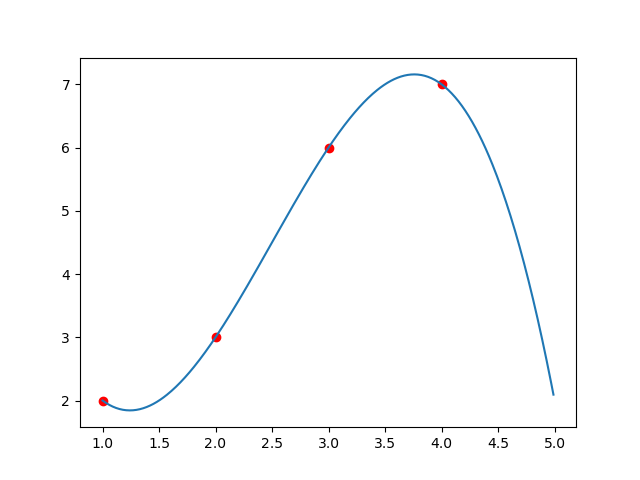
\includegraphics[width=1\linewidth]{Chapter2/graph/python/Figure2-1.png}
    \caption{Lagrange多项式插值(使用上述代码生成)}
    \label{fig:Lagrange多项式插值}
\end{figure}

\subsection{插值余项}

使用$L_n(x)$近似表示$f(x)$, 则会引起截断误差. 其截断误差为$R_n(x)=f(x)-L_n(x)$. 通常会称$R_n(x)$为插值多项式的\emph{余项}或简称为\emph{插值余项}.

为估计插值余项, 有如下定理:

\begin{theorem}
    设$f^{(n)}(x)$在$[a,b]$上连续, $f^{(n+1)}(x)$在$(a,b)$存在, 节点$a\le x_0<x_1<\cdots<x_n\le b$, $L_n(x)$是满足条件式(\ref{eqn:2.2.8})的插值多项式, 则对于任何$x\in[a,b]$, 插值余项
    \begin{equation}\label{eqn:2.2.14}
        R_n(x)=f(x)-L_n(x)=\frac{f^{(n+1)}(\xi)}{(n+1)!}\prod_{i=0}^n(x-x_i)
    \end{equation}
    其中, $\xi\in(a,b)$且依赖于$x$
\end{theorem}

\begin{proof}
    由插值条件可知, $R_n(x)$在节点$x_k,k=0,1,\cdots,n$上为0,即可以做因式分解
    \begin{equation*}
        R_n(x)=K(x)(x-x_0)(x-x_1)\cdots(x-x_n)=K(x)\prod_{i=0}^n(x-x_i)
    \end{equation*}
    其中, $K(x)$是与$x$有关的待定系数.

    把$x$视作区间$[a,b]$上的一个固定点, 作函数
    \begin{equation*}
        \varphi(t)=f(t)-L_n(t)-K(t)(t-x_0)(t-x_1)\cdots(t-x_n)
    \end{equation*}
    因此, $\varphi(t)$在$x_0,x_1,\cdots,x_n$和$x$处均为0, 即在区间$[a,b]$上有$n+2$个零点. 根据Roll定理可知, $\varphi'(t)$在两个零点间至少有一个零点, 即在区间$[a,b]$上, $\varphi'(t)$至少有$n+1$个零点. 以此类推, 不难得$\varphi^{(n+1)}$在区间$(a,b)$内至少有一个零点, 将其记为$\xi\in(a,b)$, 使得
    \begin{equation*}
        \varphi^{(n+1)}(\xi)=f^{(n+1)}(\xi)-(n+1)!K(x)=0
    \end{equation*}
    整理可得
    \begin{equation*}
        K(x)=\frac{f^{(n+1)}(\xi)}{(n+1)!}, \xi\in(a,b)
    \end{equation*}

    将其代入上式, 可得余项表达式(\ref{eqn:2.2.14})
\end{proof}

通常, $\xi$无法具体确定, 从而实际操作中, 经常估计误差上限. 由
\begin{equation*}
    \abs{f^{(n+1)}(x)}\le M_{n+1}
\end{equation*}
对于任意的$x\in(a,b)$, 将
\begin{equation*}
    \frac{M_{n+1}}{(n+1)!}\prod_{i=0}^n\abs{x-x_i}
\end{equation*}
作为误差估计上限. 通常取
\begin{equation*}
    M_{n+1}=\max_{a\le x\le b}\abs{f^{(n+1)}(x)}
\end{equation*}
特别的, 若$f(x)$为任一次数小于等于$n$的多项式, 即$f(x)\in H_n\in\spn{1,x,x^2,\cdots,x^n}$, 此时$f^{(n+1)}\equiv0$, 即$R_n(x)\equiv 0$. 因此, 插值多项式对于次数小于等于$n$的多项式总是精确的.

\begin{example}
    设有$x_0\ne x_1\ne x_2\ne x_3\ne x_4$, 且$l_i(x),i=0,1,2,3,4$为Lagrange插值基函数. 求
    \begin{equation*}
        \sum_{i=0}^4\left(3x_i^4+4x_i^2+2x_i+1\right)l_i(x)
    \end{equation*}
\end{example}

\begin{solution}
    设函数$f(x)=3x^4+4x^2+2x+1$, 则
    \begin{equation*}
        \text{原式}=\sum_{i=0}^4f(x_i)l_i(x)=f(x)
    \end{equation*}
\end{solution}

\begin{example}
    已知$\sin\frac{\pi}{6}=\frac{1}{2},\sin\frac{\pi}{4}=\frac{\sqrt{2}}{2},\sin\frac{\pi}{3}=\frac{\sqrt{3}}{2}$, 利用$\sin{x}$的一次, 二次Lagrange插值, 计算$\sin{50^\circ}$并估计误差
\end{example}

% 未完成
\begin{solution}
    当$n=1$时, 利用$x_0, x_1$, 有
    \begin{align*}
        \Rightarrow &L_1(x)=\frac{x-\frac{\pi}{4}}{\frac{\pi}{6}-\frac{\pi}{4}}\cdot\frac{1}{2}+\frac{x-\frac{\pi}{6}}{\frac{\pi}{4}-\frac{\pi}{6}}\cdot\frac{\sqrt{2}}{2}\\
        \Rightarrow &L_1(\frac{5}{18}\pi)\approx0.77614
    \end{align*}
    其误差
    \begin{equation*}
        R_1(x)=\frac{f''(\xi)}{2!}\abs{x-\frac{\pi}{6}}\abs{x-\frac{\pi}{4}}
    \end{equation*}
    其中$\abs{\sin{\xi}}\le\frac{\sqrt{2}}{2}$, 因此有
    \begin{equation*}
        \abs{R_1(\frac{5}{18}\pi)}<0.01319
    \end{equation*}

    类似地, 利用$x_1,x_2$, 可得$L_1(x)\approx0.76008$, 估计误差, 由于$\abs{\sin{\xi}}\le\frac{\sqrt{3}}{2}$
    \begin{equation*}
        \abs{R_1(\frac{5}{18}\pi)}<0.00660
    \end{equation*}

    当$n=2$时,有
\end{solution}

% 事后估计

\subsection{Lagrange插值优缺点}

优点: 具有严格的规律性, 便于记忆与理论推导;

缺点: 计算量大, 每次添加(或删除)节点都需要重新计算基函数, 不具有承袭性.

为解决上述缺点, 将引出新的插值法, 即Newton插值.

\section{Newton插值}

\subsection{Newton插值}

与Lagrange插值类似, 首先考虑$n=1$

\begin{example}
    已知两个节点$x_0,x_1$, 其函数值分别为$y_0,y_1$, 试求一次多项式$P_1(x)=A_0+A_1x$, 使得$P_1(x_0)=y_0, P_1(x_1)=y_1$
\end{example}

\begin{solution}
    利用直线方程点斜式, 可知
    \begin{equation*}
        P_1(x)=y_0+\frac{y_1-y_0}{x_1-x_0}(x-x_0)
    \end{equation*}

    此时, 插值节点为$x_0,x_1$, 基函数设为$1,(x-x_0)$, 组合系数为$A_0=y_0, A_1=\frac{y_1-y_0}{x_1-x_0}$
\end{solution}

考虑$n=2$的情况, 要求具有承袭性. 设$g(x)=P_2(x)-P_1(x)$, 则$g(x)$为次数不超过2的多项式, 且有
\begin{equation*}
    g(x_i)=P_2(x_i)-P_1(x_i)=y_i-y_i=0, i=0,1
\end{equation*}
因此可对其进行因式分解, 有
\begin{align*}
    g(x)&=A_2(x-x_0)(x-x_1)\\
    \Rightarrow  P_2(x)=P_1(x)+A_2(x-x_0)(x-x_1)
\end{align*}

故, 对于$n=2$而言, 插值节点为$x_0,x_1,x_2$, 基函数为$1,(x-x_0),(x-x_0)(x-x_1)$, 组合系数为$A_0,A_1,A_2$. 插值多项式为
\begin{equation*}
    P_2(x)=A_0+A_1(x-x_0)+A_2(x-x_0)(x-x_1)
\end{equation*}

类似地, 给定插值条件
\begin{equation*}
    N_n(x_i)=f(x_i), i=0,1,\cdots,n
\end{equation*}
, 插值节点为$x_i, i=0,1,\cdots,n$, 基函数为$1,(x-x_0),(x-x_0)(x-x_1),\cdots,(x-x_0)(x-x_1)\cdots(x-x_{n-1})$, 组合系数为$A_i,i=0,1,\cdots,n$

下面需要讨论如何求解组合系数.

设$A_n(x)=A_0+A_1(x)(x-x_0)+A_2(x-x_0)(x-x_1)+\cdots+A_n(x-x_0)(x-x_1)\cdots(x-x_n)$, 利用插值条件
\begin{equation*}
    N_n(x_i)=f(x_i),i=0,1,\cdots,n
\end{equation*}
代入, 得线性方程组
\begin{equation*}
    \mqty(1&0&\cdots&0\\1&x_1-x_0&\cdots&0\\\vdots&\vdots&&\vdots\\1&x_n-x_0&\cdots&\prod_{i=0}^{n-1}(x_n-x_i))\mqty(A_0\\A_1\\\vdots\\A_n)=\mqty(f(x_0)\\f(x_1)\\\vdots\\f(x_n))
\end{equation*}

求解方程组, 可得
\begin{align*}
    A_0&=f(x_0)\\
    A_1&=\frac{f(x_1)-f(x_0)}{x_1-x_0}\\
    A_2&=\frac{\frac{f(x_2)-f(x_0)}{x_2-x_0}-\frac{f(x_1)-f(x_0)}{x_1-x_0}}{x_2-x_1}\\
    &\vdots
\end{align*}

为简化计算, 总结上述规律, 给出下面关于\emph{差商}的定义

\subsection{差商}

\subsubsection{差商的定义}

\begin{definition}[差商]
    称
    \begin{equation*}
        f[x_0,x_k] = \frac{f(x_k)-f(x_0)}{x_k-x_0}
    \end{equation*}
    为函数$f(x)$关于点$x_0,x_k$的\emph{一阶差商}, 称
    \begin{equation*}
        f[x_0,x_1,x_k]=\frac{f[x_0,x_k]-f[x_0,x_1]}{x_k-x_1}
    \end{equation*}
    为$f(x)$关于点$x_0,x_1,x_k$的\emph{二阶差商}. 一般地, 称
    \begin{equation*}
        f[x_0,x_1,\cdots,x_k]=\frac{f[x_0,x_1,\cdots,x_{k-2},x_k]-f[x_0,x_1,\cdots,x_{k-1}]}{x_k-x_{k-1}}
    \end{equation*}
    为$f(x)$的\emph{$k$阶差商}.
\end{definition}

由差商定义可知: \emph{高阶差商是两个低一阶差商的差商}.

利用差商定义, 可知组合系数为:
\begin{align*}
    A_0&=f(x_0)=f[x_0]\\
    A_1&=f[x_0,x_1]\\
    &\vdots\\
    A_n&=f[x_0,x_1,\cdots,x_n]
\end{align*}
\begin{align*}
    \Rightarrow N_n(x)=&f(x_0)+f[x_0,x_1](x-x_0)+f[x_0,x_1,x_2](x-x_0)(x-x_1)\\
    &+\cdots+f[x_0,x_1,\cdots,x_n](x-x_0)(x-x_1)\cdots(x-x_{n-1})
\end{align*}

\subsubsection{差商性质}

差商与函数值有如下关系:

\begin{theorem}
    记$\omega(x)=(x-x_0)(x-x_1)\cdots(x-x_n)$, 则
    \begin{equation*}
        f[x_0,x_1,\cdots,x_n]=\sum_{i=0}^n\frac{f(x_i)}{\omega'(x_i)}
    \end{equation*}
\end{theorem}

\begin{proof}
    对于$f(x)$, 使用Lagrange插值法, 可得:
    \begin{equation*}
        L_n(x)=\sum_{i=0}^nf(x_i)l_i(x)
    \end{equation*}
    使用Newton插值法, 可得:
    \begin{equation}\label{eqn:2.4.6}
        N_n(x)=f(x_0)+f[x_0,x_1](x-x_0)+\cdots+f[x_0,x_1,\cdots,x_n](x-x_0)(x-x_1)\cdots(x-x_{n-1})
    \end{equation}

    由于插值多项式具有唯一性, 因此两种插值方法得到的结果相同, 即同次系数相等. 整理可得
    \begin{equation*}
        \sum_{i=0}^nf(x_i)=f[x_0,x_1,\cdots,x_n](x-x_0)(x-x_1)\cdots(x-x_{n-1})
    \end{equation*}
    对$\omega(x)$求导后, 原式得证.
\end{proof}

差商的值与节点的排列顺序无关, 即\emph{差商具有对称性}. 用公式表示为:
\begin{equation*}
    f[x_0,\cdots,x_i,\cdots,x_j\cdots,x_n]=f[x_0,\cdots,x_j,\cdots,x_i\cdots,x_n]
\end{equation*}

设$f(x)$在$[a,b]$有$n$阶导数, 且$x_0,x_1,\cdots,x_n\in[a,b]$, 则存在$\xi\in(a,b)$, 使得
\begin{equation*}
    f[x_0,x_1,\cdots,x_n]=\frac{f^{(n)}(\xi)}{n!}
\end{equation*}

\begin{example}
    若$f(x)=3x^4+4x^2+2x+1$, 计算
    \begin{equation*}
        f[2^0,2^1,2^2,2^3,2^4], f[2^0,2^1,2^2,2^3,2^4,2^5]
    \end{equation*}
\end{example}

\begin{solution}
    \begin{align*}
        f[2^0,2^1,2^2,2^3,2^4]&=\frac{f^{(4)}(\xi)}{4!}=3\\
        f[2^0,2^1,2^2,2^3,2^4,2^5]&=\frac{f^{(5)}(\xi)}{5!}=0
    \end{align*}
\end{solution}

由前面的性质, 不难得到, 对于差商而言, 有
\begin{equation*}
    f[x_0.x_1,\cdots,x_n]=\frac{f[x_1,x_2,\cdots,x_n]-f[x_0,x_1,\cdots,x_{n-1}]}{x_n-x_0}
\end{equation*}

该性质表明在实际计算差商过程中, 可以使用列表法计算.

\subsection{Newton插值余项}

\begin{theorem}%待证明
    Newton插值多项式的余项为:

    \begin{equation*}
        R_n(x)=f[x_0,x_1,\cdots,x_n]\omega_{n+1}(x)
    \end{equation*}
    其中,
    \begin{equation*}
        \omega_{n+1}(x)=(x-x_0)(x-x_1)\cdots(x-x_n)=\prod_{i=0}^n(x-x_i)
    \end{equation*}
\end{theorem}

\section{等距节点差商公式}

\subsection{差分定义}

\begin{definition}[差分]
    设函数$y=f(x)$在等距节点$x_k=x_0+kh(k=0,1,\cdots,n)$上的值$f_k=f(x_k)$已知, 其中$h$为常数, 称为\emph{步长}, 称偏差

    \begin{align*}
        \Delta f_k&=f_{k+1}-f_k\\
        \nabla f_k&=f_k-f_{k-1}\\
        \delta f_k&=f(x_k+h/2)-f(x_k-h/2)=f_{k+\frac{1}{2}}-f_{k-\frac{1}{2}}\\
    \end{align*}
    分别称为$f(x)$在$x_k$处以$h$为步长的\emph{向前差分, 向后差分, 中心差分}. 符号$\Delta, \nabla, \delta$分别称为\emph{向前差分算子, 向后差分算子, 中心差分算子}.
\end{definition}

利用一阶差分, 类似可定义二阶差分为
\begin{equation*}
    \Delta^2f_k=\Delta f_{k+1}-\Delta f_k=f_{k+2}-2f_{k+1}+f_k
\end{equation*},
一般地, $m$阶差分为
\begin{equation*}
    \Delta^mf_k=\Delta^{m-1}f_{k+1}-\Delta^{m-1}f_k
\end{equation*}

\subsection{差分的性质}

定义不变算子$I$和移位算子$E$, 即有
\begin{equation*}
    If_k=f_k, Ef_k=f_{k+1}
\end{equation*}
由差分定义, 可得$\Delta=E-I, \nabla=I-E^{-1}, \delta=E^{\frac{1}{2}}-E^{-\frac{1}{2}}$

由不变算子和移位算子, 可得如下性质:

各阶差分均可用函数值表示, 即

\begin{align*}
    \Delta^nf_k&=(E-1)^nf_k=\sum_{j=0}^n(-1)^j\mqty(n\\j)E^{n-j}f_k=\sum_{j=0}^n(-1)^j\mqty(n\\j)f_{n+k-j}\\
    \nabla^nf_k&=(1-E^{-1})^nf_k=\sum_{j=0}^n(-1)^{n-j}\mqty(n\\j)E^{j-n}f_k=\sum_{j=0}^n(-1)^{n-j}\mqty(n\\j)f_{k+j-n}
\end{align*}
其中$\mqty(n\\j)=\frac{n(n-1)\cdots(n-j+1)}{j!}$为二项式展开系数

差商与差分之间满足下面的关系. 例如, 对于向前差分, 由定义
\begin{align*}
    f[x_k,x_{k+1}]&=\frac{f_{k+1}-f_k}{x_{k+1}-x_k}=\frac{\Delta f_k}{h}\\
    f[x_k,x_{k+1},x_{k+2}]&=\frac{f[x_{k+1},x_{k+2}]-f[x_k,x_{k+1}]}{x_{k+2}-x_k}=\frac{1}{2h^2}\Delta^2f_k
\end{align*}
一般有
\begin{equation}\label{eqn:2.5.7}
    f[x_k,x_{k+1},\cdots,x_{k+m}]=\frac{1}{m!}\frac{1}{h^m}\Delta^mf_k, m=1,2,\cdots,n
\end{equation}

同理, 对于向后差分, 有
\begin{equation}\label{eqn:2.5.8}
    f[x_k,x_{k-1},\cdots,x_{k-m}]=\frac{1}{m!}\frac{1}{h^m}\nabla^mf_k
\end{equation}

利用差商的导数关系, 可得差分与导数的关系为
\begin{equation*}
    \Delta^nf_k=j^nf^{(n)}(\xi)
\end{equation*}

\subsection{等距节点插值公式}

利用Newton插值公式, 将差商用相应的差分替代, 即可得到等距节点插值公式. 

若节点$x_k=x_0+kh, k=0,1,\cdots,n$, 要计算$x_0$附近点$x$的函数$f(x)$的值, 令$x=x_0+th$, 其中$0\le t\le1$, 于是有
\begin{equation*}
    \omega_{k+1}(x)=\prod_{j=0}^k(x-x_j)=t(t-1)\cdots(t-k)h^{k+1}
\end{equation*}

将该式与式(\ref{eqn:2.5.7})代入公式(\ref{eqn:2.4.6}), 可得
\begin{equation*}
    N_n(x_0+th)=f_0+t\Delta f_0+\frac{t(t-1)}{2!}\Delta^2f_0+\cdots+\frac{t(t-1)\cdots(t-n+1)}{n!}\Delta^nf_0
\end{equation*}
上式称为\emph{Newton前插公式}. 同时, 由于其使用$x_0$附近的点, 故又称为\emph{表初公式}.

不难得到, 上式的余项可由式(\ref{eqn:2.2.14})得到
\begin{equation*}
    R_n(x)=\frac{t(t-1)\cdots(t-n)}{(n+1)!}h^{n+1}f^{(n+1)}(\xi), \xi\in(x_0,x_n)
\end{equation*}

类似地, 若要计算$x_n$附近的值$f(x)$, 则可将Newton插值公式(\ref{2.4.6})按照倒序排列, 即$x_n,x_{n-1},\cdots,x_0$的次序. 此时有

\begin{align*}
    N_n(x)=&f(x_n)+f[x_n,x_{n-1}](x-x_n)+f[x_n,x_{n-1},x_{n-2}](x-x_n)(x-x_{n-1})\\
    &+\cdots+f[x_n,x_{n-1},\cdots,x_0](x-x_n)\cdots(x-x_1)
\end{align*}

变换$x=x_n-th(-1\le t\le0)$, 并利用公式(\ref{eqn:2.5.8}), 代入可得
\begin{equation*}
    N_n(x_n+th)=f_n+t\nabla f_n+\frac{t(t+1)}{2!}\nabla^2f_n+\cdots+\frac{t(t+1)\cdots(t+n-1)}{n!}\nabla^nf_n
\end{equation*}

上式称为\emph{Newton后插公式}或\emph{表末公式}. 其余项为
\begin{equation*}
    R_n(x)=f(x)-N_n(x_n+th)=\frac{t(t+1)\cdots(t+n)h^{n+1}f^{(n+1)}(\xi)}{(n+1)!}, \xi\in(x_0,x_n)
\end{equation*}

\section{Hermite插值}

\subsection{引入, Hermite插值多项式的存在唯一性}
在有些情况下, 不仅要求节点上函数值相等, 同时\emph{要求节点上导数值相等, 甚至要求高阶导数值相等}. 满足该要求的插值多项式就是\emph{Hermite插值多项式}.

仅讨论函数值与导数值个数相等情况. 设在节点$a\le x_0<x_1<\cdots<x_n\le b$上, $y_i=f(x_i), m_i=f'(x_i)(i=0,1,\cdots,n)$, 要求插值多项式$H(x)$满足条件
\begin{equation*}
    H(x_i)=y_i, H'(x_i)=m_i, (i=0,1,\cdots,n)
\end{equation*}
给出$(2n+2)$个条件, 可唯一确定一个次数不超过$2n+1$的多项式$H_{2n+1}$, 其形式为
\begin{equation*}
    H_{2n+1}(x)=a_0+a_1x+\cdots+a_{2n+1}x^{2n+1}
\end{equation*}

\subsection{Hermite插值多项式构造}

\subsubsection{Lagrange型Hermite插值多项式}
先求插值基函数$\alpha_i(x)$和$\beta_i(x),i=0,1,\cdots,n$, 共有$2n+2$个, 每一个都是$2n+1$次多项式, 且满足条件:
\begin{equation*}
    \begin{cases}
        \alpha_i(x_k)=\delta_{ik}=
        \begin{cases}
            0, j\ne k,\\
            1, j=k,
        \end{cases}, \alpha'_i(x_k)=0\\
        \beta_i(x_k)=0, \beta'_i(x_k)=\delta_{ik}
    \end{cases}
\end{equation*}

因此, 满足插值条件的插值多项式$H(x)=H_{2n+1}(x)$可用插值基函数表示为
\begin{equation*}
    H_{2n+1}(x)=\sum_{i=0}^n\left[y_i\alpha_i(x)+m_i\beta_i(x)\right]
\end{equation*}
显然有
\begin{equation*}
    H_{2n+1}(x_k)=y_k, H'_{2n+1}(x_k)=m_k, k=0,1,\cdots,n
\end{equation*}

为构造基函数, 使用Lagrange插值基函数$l_i(x)$, 令
\begin{equation*}
    \alpha_i(x)=(ax+b)l_i^2(x)
\end{equation*}
其中$l_i(x)$是式(\ref{2.2.10})所表示的基函数. 由上述条件, 有
\begin{align*}
    \alpha_i(x_i)&=(ax_i+b)l_i^2(x_i)=1,\\
    \alpha'_i(x_i)&=l_i(x_i)\left[al_i(x_i)+2(ax_i+b)l'_i(x_i)\right]=0
\end{align*}
整理可得
\begin{equation*}
    \begin{cases}
        ax_i+b=1\\
        a+2l'_i(x_i)=0
    \end{cases}
\end{equation*}
解得
\begin{equation*}
    a=-2l'_i(x_i), b=1+2x_il'_i(x_i)
\end{equation*}

由于
\begin{equation*}
    l_i(x)=\frac{(x-x_0)\cdots(x-x_{i-1})(x-x_{i+1})\cdots(x-x_n)}{(x_i-x_0)\cdots(x_i-x_{i-1})(x_i-x_{i+1})\cdots(x_i-x_n)}
\end{equation*}
取对数后求导, 得
\begin{equation*}
    l_i'(x_i)=\sum_{\substack{k=0\\k\ne i}}^n\frac{1}{x_i-x_k}
\end{equation*}
于是可得
\begin{equation}\label{eqn:2.6.4}
    \alpha_i(x)=\left[1-2(x-x_i)\sum_{\substack{k=0\\k\ne i}}^n\frac{1}{x_i-x_k}\right]l_i^2(x)
\end{equation}
同理可得
\begin{equation}\label{eqn:2.6.5}
    \beta_i(x)=(x-x_i)l_i^2(x)
\end{equation}

\begin{extend}
    下面证明\emph{满足插值条件得插值多项式是唯一的}.

    \begin{proof}
        使用反证法, 设$H_{2n+1}(x)$和$\overline{H}_{2n+1}(x)$均满足条件, 则有
        \begin{equation*}
            \varphi(x)=H_{2n+1}(x)-\overline{H}_{2n+1}(x)
        \end{equation*}
        其在每个节点上均有二重根, 故$\varphi(x)$有$2n+2$重根, 但$\varphi(x)$是不高于$2n+1$次的多项式, 故$\varphi\equiv0$.

        唯一性得证.
    \end{proof}
\end{extend}

利用Lagrange插值余项证明方法, 可得若$f(x)$在$(a,b)$内的$2n+2$阶导数存在, 则插值余项为
\begin{equation}\label{eqn:2.6.6}
    R(x)=f(x)-H_{2n+1}(x)=\frac{f^{(2n+2)}(\xi)}{(2n+2)!}\omega_{n+1}^2(x)
\end{equation}
其中$\xi\in(a,b)$且与$x$有关.

考虑特殊情况$n=1$, 取节点为$x_k,x_{k+1}$, 插值多项式为$H_3(x)$, 满足条件
\begin{equation}\label{eqn:2.6.7}
    \begin{cases}
        H_3(x_k)=y_k, H_3(x_{k+1})=y_{k+1}\\
        H_3'(x_k)=m_k, H_3'(x_{k+1})=m_{k+1}
    \end{cases}
\end{equation}
相应的插值基函数为$\alpha_k(x),\alpha_{k+1}(x),\beta_k(x),\beta_{k+1}(x)$, 且满足条件
\begin{gather*}
    \alpha_k(x_k)=1,\alpha_k(x_{k+1})=0, \alpha_k'(x_k)=\alpha_k'(x_{k+1})=0,\\
    \alpha_{k+1}(x_k)=0,\alpha_{k+1}(x_{k+1})=1,\\
    \alpha_{k+1}'(x_k)=\alpha_{k+1}'(x_{k+1})=0,\\
    \beta_k(x_k)=\beta_k(x_{k+1})=0,\\
    \beta_k'(x_k)=1,\beta_k'(x_{k+1})=0,\\
    \beta_{k+1}(x_k)=\beta_{k+1}(x_{k+1})=0,\\
    \beta_{k+1}'(x_k)=0,\beta_{k+1}'(x_{k+1})=1
\end{gather*}

根据式(\ref{eqn:2.6.4})和(\ref{eqn:2.6.5}), 可得
\begin{gather*}
    \begin{cases}
        \alpha_k(x)=\left(1+2\frac{x-x_k}{x_{k+1}-x_k}\right)\left(\frac{x-x_{k+1}}{x_k-x_{k+1}}\right)^2,\\
        \alpha_{k+1}(x)=\left(1+2\frac{x-x_{k+1}}{x_k-x_{k+1}}\right)\left(\frac{x-x_{k}}{x_{k+1}-x_{k}}\right)^2;
    \end{cases}\\
    \begin{cases}
        \beta_k(x)=(x-x_k)\left(\frac{x-x_{k+1}}{x_k-x_{k+1}}\right)^2,\\
        \beta_{k+1}(x)=(x-x_{k+1})\left(\frac{x-x_k}{x_{k+1}-x_k}\right)^2
    \end{cases}
\end{gather*}
满足式(\ref{eqn:2.6.7})的插值多项式是
\begin{equation*}
    H_3(x)=y_k\alpha_k(x)+y_{k+1}\alpha_{k+1}(x)+m_k\beta_k(x)+m_{k+1}\beta_{k+1}(x)
\end{equation*}
由式(\ref{eqn:2.6.6})可得其余项为
\begin{equation*}
    R_3(x)=\frac{1}{4!}f^{(4)}(\xi)(x-x_k)^2(x-x_{k+1})^2
\end{equation*}

\subsubsection{Newton型Hermite插值多项式}

若给定插值条件
\begin{equation*}
    H(x_0)=f(x_0),H'(x_0)=f'(x_0),\cdots,H^{(m)}(x_0)=f^{(m)}(x_0)
\end{equation*}

利用Newton插值法, 其节点为$x_0,x_0,\cdots,x_0$, 基函数分别为$1,(x-x_0),(x-x_0)^2,\cdots,(x-x_0)^m$, 组合系数为$f(x_0),f[x_0,x_0],\cdots,f[x_0,x_0,\cdots,x_0]$

考虑差商与导数的性质, 有
\begin{equation*}
    f[x_0,x_0,\cdots,x_0]=\frac{f^{(n)}}{n!}
\end{equation*}
故容易得到, Newton型Hermite插值多项式为
\begin{equation*}
    H(x)=f(x_0)+f'(x_0)(x-x_0)+\cdots+\frac{f^{(m)}}{m!}(x-x_0)^m
\end{equation*}

\begin{example}
    给定函数表
    \begin{table}[h]
        \centering
        \begin{tabular}{|c|c|c|c|}
            $x_i$&3&4&6\\
            \hline
            $y_i$&6&0&2\\
            \hline
            $y_i'$&1&&-1\\
        \end{tabular}
    \end{table}
    求插值多项式$P_4(x)$
\end{example}

\begin{solution}
    利用Newton法, 列差商表如下所示
    \begin{table}[h]\label{tab:1}
        \centering
        \caption{差商表}
        \begin{tabular}{|c|c|c|c|c|c|}
            $x_k$&$f(x_k)$&一阶差商&二阶差商&三阶差商&四阶差商\\
            \hline
            3&6& & & & \\
            3&6&$f[3,3]=1$& & &\\
            4&0&$f[3,4]$&$f[3,3,4]$& &\\
            6&2&$f[4,6]$&$f[3,4,6]$&$f[3,3,4,6]$&\\
            6&2&$f[6,6]=-1$&$f[4,6,6]$&$f[3,4,6,6]$&$f[3,3,4,6,6]$\\
        \end{tabular}
    \end{table}
    将差商表计算可得
    \begin{equation*}
        P_4=6+1(x-3)+(-7)(x-3)^2+\frac{28}{9}(x-3)^2(x-4)+\left(-\frac{38}{27}\right)(x-3)^2(x-4)(x-6)
    \end{equation*}
    其插值余项为
    \begin{equation*}
        R_4(x)=f[3,3,4,6,6,x](x-3)^2(x-4)(x-6)^2
    \end{equation*}
\end{solution}

\section{分段低次插值}

\subsection{多项式插值的Runge现象}

\begin{example}
    在$[-5,5]$考察函数
    \begin{equation*}
        f(x)=\frac{1}{1+x^2}
    \end{equation*}
    的$L_n(x)$
\end{example}

使用下面的代码:

\begin{lstlisting}
# Runge现象演示 Exercise2-3.py

import numpy as np
import matplotlib.pyplot as plt
from scipy.interpolate import lagrange

# 定义函数
def f(x):
    return 1 / (1 + x ** 2)

# 生成插值节点
n = 11
x = np.linspace(-5, 5, n)
y = f(x)

# 生成插值多项式
poly = lagrange(x, y)

# 生成等距节点
x_interp = np.linspace(-5, 5, 1000)
y_interp = f(x_interp)

# 生成插值函数
y_poly = poly(x_interp)

# 绘图
plt.plot(x_interp, y_interp)
plt.plot(x_interp, y_poly)
plt.plot(x, y, 'o')
plt.show()
\end{lstlisting}

生成图像如图(\ref{fig:Runge现象})所示
\begin{figure}[h]
    \centering
    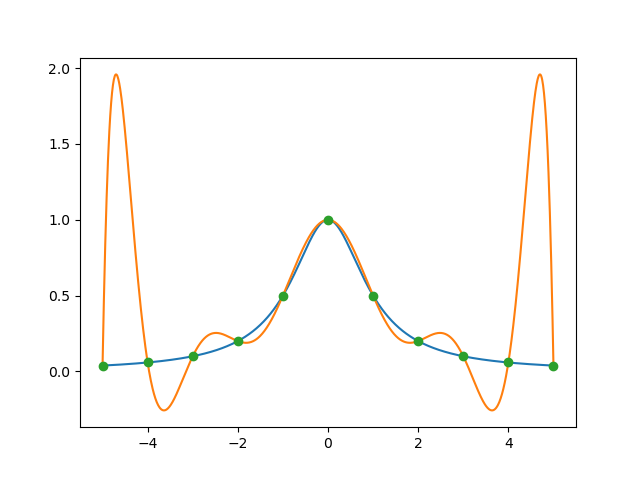
\includegraphics[width=1\linewidth]{Chapter2/graph/python/Figure2-2.png}
    \caption{Runge现象}
    \label{fig:Runge现象}
\end{figure}

可以看到, 随着节点的增多, 插值多项式在节点处出现振荡. 这就是多项式插值的\emph{Runge现象}. 为解决这一问题, 采用分段插值的方法.

\subsection{分段线性插值}

在每个区间$[x_i,x_{i+1}]$上, 用一阶多项式逼近$f(x)$, 即
\begin{equation*}
    f(x)=P_1(x)=\frac{x-x_{i+1}}{x_i-x_{i+1}}y_i+\frac{x-x_i}{x_{i+1}-x_i}y_{i+1}, x\in[x_i,x_{i+1}]
\end{equation*}

若用插值基函数表示, 若整个节点在$[a,b]$之间, 则在整个区间的$P_1(x)$可以表示为
\begin{equation*}
    P_1(x)=\sum_{i=0}^ny_il_i(x)
\end{equation*}
其中$l_i(x)$满足条件$l_i(x_k)=\delta_{ik}, i,k=0,1,\cdots,n$, 其形式为
\begin{equation*}
    l_i(x)=
    \begin{cases}
        \frac{x-x_{i-1}}{x_i-x_{i-1}}, &x_{i-1}\le x\le x_i(i=0\text{略去}),\\
        \frac{x_i-x_{i+1}}{x-x_{i+1}}, &x_i\le x\le x_{i+1}(i=n\text{略去}),\\
        0, &x\in[a,b], x\notin[x_{i-1},x_{i+1}].
    \end{cases}
\end{equation*}

不难发现, 基函数$l_i(x)$在$x_i$附近不为0, 其他地方均为零, 这种性质称为\emph{局部非零性质}.

关于分段线性插值的误差估计, 给出如下定理(暂不做证明)% 待证明

\begin{theorem}
    若$f(x)$在$[a,b]$上二阶连续可微, 则分段线性插值$P(x)$余项有如下估计:
    \begin{equation*}
        \abs{R(x)}=\abs{f(x)-P(x)}\le\frac{h^2}{8}M
    \end{equation*}
    其中,
    \begin{align*}
        h&=\max_{0\le i\le n-1}\left(x_{i+1}-x_i\right)\\
        M&=\max_{a\le x\le b}\abs{f''(x)}
    \end{align*}
\end{theorem}

下面的程序, 演示了分段线性插值(图像如图\ref{fig:分段线性插值}所示). 可以看到, 分段线性插值\emph{在节点处不光滑}. 为了改善该问题, 我们可以借助于Hermite插值, 即下面的\emph{分段三次Hermite插值}.

\begin{lstlisting}
# 分段线性插值演示 Exercise2-4.py

import numpy as np
import matplotlib.pyplot as plt

# 定义函数
def f(x):
    return np.sin(x)

# 生成插值节点
n = 6
x = np.linspace(0, 2*np.pi, n)
y = f(x)

# 生成分段线性插值函数
x_interp = np.linspace(0, 2*np.pi, 1000)
y_interp = np.zeros_like(x_interp)
for i in range(len(x_interp)):
    if x_interp[i] <= x[0]:
        y_interp[i] = y[0]
    elif x_interp[i] >= x[-1]:
        y_interp[i] = y[-1]
    else:
        j = np.searchsorted(x, x_interp[i])
        x_left = x[j-1]
        x_right = x[j]
        y_left = y[j-1]
        y_right = y[j]
        slope = (y_right - y_left) / (x_right - x_left)
        y_interp[i] = y_left + slope * (x_interp[i] - x_left)

# 绘图
plt.plot(x_interp, f(x_interp))
plt.plot(x_interp, y_interp)
plt.plot(x, y, 'o')
plt.show()
\end{lstlisting}

\begin{figure}[h]
    \centering
    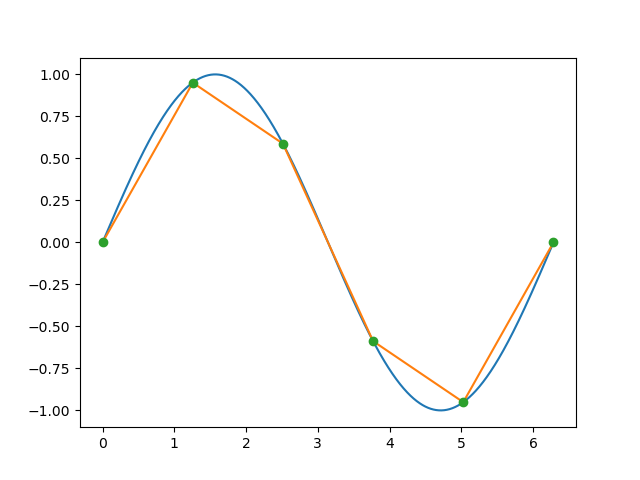
\includegraphics[width=1\linewidth]{Chapter2/graph/python/Figure2-3.png}
    \caption{$\sin{x}$的分段线性插值}
    \label{fig:分段线性插值}
\end{figure}

\subsection{分段三次Hermite插值}

给定节点$a\le x_0<x_1<\cdots\le b$, $f(x)$在节点$x_i$上的函数值及导数值分别为$y_i,m_i$. 在每个子区间$[x_i,y_i]$上作两点三次Hermite插值, 插值函数为
\begin{equation}\label{eqn:2.7.6}
    H(x)=\sum_{i=0}^n\left[y_i\varphi_i(x)+m_i\psi_i(x)\right]
\end{equation}
其中基函数为
\begin{align*}
    \varphi_i(x)&=
    \begin{cases}
        \left(\frac{x-x_{i-1}}{x_i-x_{i-1}}\right)^2\left(1+2\frac{x-x_i}{x_{i-1}-x_i}\right),&x_{i-1}\le x\le x_i,\\
        \left(\frac{x-x_{i+1}}{x_i-x_{i+1}}\right)^2\left(1+2\frac{x-x_i}{x_{i+1}-x_i}\right),&x_i\le x\le x_{i+1},\\
        0,&x\notin[x_{i-1},x_{i+1}]
    \end{cases}, (i=1,2,\cdots,n-1).\\
    \psi_i(x)&=
    \begin{cases}
        (x-x_i)\left(\frac{x-x_{i-1}}{x_i-x_{i-1}}\right)^2,&x_{i-1}\le x\le x_i,\\
        (x-x_i)\left(\frac{x-x_{i+1}}{x_i-x_{i+1}}\right)^2,&x_{i}\le x\le x_{i+1},\\
        0,&x\notin[x_{i-1},x_{i+1}]
    \end{cases}
\end{align*}

由三次Hermite插值的余项可以估计分段Hermite插值的余项. 设$H(x)$是给定节点
\begin{equation*}
    a=x_0<x_1<\cdots<x_n=b
\end{equation*}
上的分段三次Hermite插值函数, $f(x)\in C^4[a,b]$, 则$f(x)$与$H(x)$的误差限为
\begin{equation*}
    \abs{R(x)}\le\abs{f(x)-H(x)}\le\frac{h^4}{384}M_4
\end{equation*}
其中,
\begin{align*}
    h&=\max_{0\le i\le n-1}\abs{x_{i+1}-x_i},\\
    M&=\max_{a\le x\le b}\abs{f^{(4)}(x)}
\end{align*}

下面的代码演示了分段三次Hermite插值, 并绘制了图\ref{fig:三次Hermite插值}. 可以看到, 与线性插值(图\ref{fig:分段线性插值})相比, 三次Hermite插值具有光滑性.

\begin{extend}
    在该代码中使用了Python的库函数PchipInterpolator(), 这个函数会在内部自动计算导数值, 因此与前面所讨论的理论在形式上可能有些许不同.
\end{extend}

\begin{lstlisting}
# 分段三次Hermite插值演示 Exercise2-5.py

import numpy as np 
import matplotlib.pyplot as plt 
from scipy.interpolate import PchipInterpolator 

# 定义函数 
def f(x): 
   return np.sin(x)
 
# 生成插值节点 
n = 5 
x = np.linspace(0, 2*np.pi, n)
y = f(x)

# 生成分段三次Hermite插值函数 
x_interp = np.linspace(0, 2*np.pi, 1000)
y_interp = PchipInterpolator(x, y)(x_interp)
 
# 绘图 
plt.plot(x_interp, f(x_interp)) 
plt.plot(x_interp, y_interp) 
plt.plot(x, y, 'o') 
plt.show()
\end{lstlisting}

\begin{figure}[h]
    \centering
    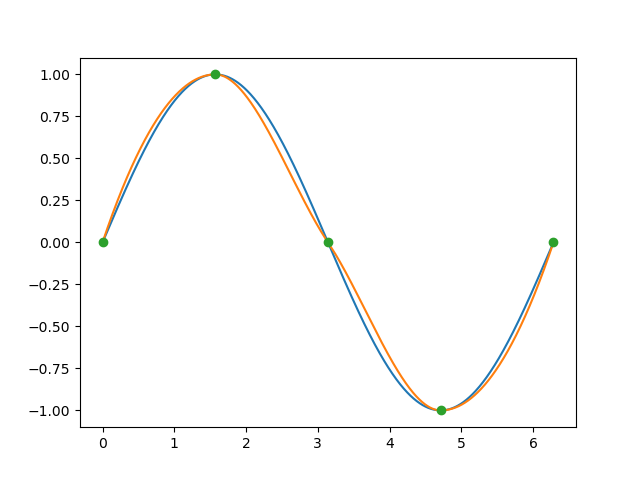
\includegraphics[width=1\linewidth]{Chapter2/graph/python/Figure2-4.png}
    \caption{$\sin{x}$的三次Hermite插值}
    \label{fig:三次Hermite插值}
\end{figure}

\section{三次样条插值}

\subsection{三次样条函数}

设对$y=f(x)$在区间$[a,b]$上给定一组节点$a=x_0<x_1<\cdots<x_n=b$和相应的函数值$y_0,y_1,\cdots,y_n$, 如果$s(x)$具有如下性质:
\begin{enumerate}
    \item 在每个子区间$[x_{i-1},x_i],i=1,2,\cdots,n$上$s(x)$是不高于三次的多项式;
    \item $s(x),s'(x),s''(x)$在$[a,b]$上连续, 则称$s(x)$是\emph{三次样条函数}. 若再有
    \item $s(x_i)=f(x_i),i=0,1,\cdots,n$, 则称$s(x)$为$y=f(x)$的\emph{三次样条插值函数}.
\end{enumerate}

\subsection{三次样条插值函数构造}

首先对三次样条插值的存在性进行证明

\begin{proof}
    设有$n$个区间, 对于每个区间$S_i$, 插值函数为
    \begin{equation*}
        S_i(x)=a_i+b_ix+c_ix^2+d_ix^3, i=0,1,\cdots,n-1
    \end{equation*}

    对于每一个小区间, 两个端点给定, 总区间共有$2n$个条件.

    对于节点$x_i$, 其一阶导数连续, 即
    \begin{equation*}
        S'_{i-1}(x_i)=S'_i(x_i)
    \end{equation*}
    共$(n-1)$个条件.

    同理, 其二阶导数连续, 有$(n-1)$个条件.

    因此, 给定条件共$(4n-2)$个, 小于$4n$, 因此解存在但不唯一.
\end{proof}

为保证解的唯一性, 需要补充边界条件. 常见的边界条件有如下四种:

固支边界条件(D-1样条):
\begin{equation*}
    \begin{cases}
        S'(x_0)=f'(x_0)=m_0\\
        S'(x_n)=f'(x_n)=m_n
    \end{cases}
\end{equation*}

弯矩边界条件(D-2样条):
\begin{equation*}
    \begin{cases}
        S''(x_0)=f''(x_0)=M_0\\
        S''(x_n)=f''(x_n)=M_n
    \end{cases}
\end{equation*}

自然边界条件(自然样条):
\begin{equation*}
    \begin{cases}
        S''(x_0)=0\\
        S''(x_n)=0
    \end{cases}
\end{equation*}

周期边界条件(周期样条):
\begin{equation*}
    \begin{cases}
        S(x_0)=S(x_n)\\
        S'(x_0)=S'(x_n)\\
        S''(x_0)=S''(x_n)
    \end{cases}
\end{equation*}

\subsection{三转角方程}

假定$S'(x)$在节点$x_i$的值为$S'(x_i)=m_i,i=0,1,\cdots,n$, 由式(\ref{eqn:2.7.6})可得
\begin{equation*}
    S(x)=\sum_{i=0}^n\left[y_i\varphi_i(x)+m_i\psi_i(x)\right]
\end{equation*}
显然, 该表达式在$[a,b]$区间连续, 且满足插值条件. 而式中的导数值$m_i$未知, 因此可利用导数的连续条件:
\begin{equation*}
    S''(x_i-0)=S''(x_i+0), i=1,2,\cdots,n-1
\end{equation*}
以及边界条件确定. 

下面考虑$S(x)$在$[x_i,x_{i+1}]$的表达式
\begin{align*}
    S(x)&=\frac{(x-x_{i+1})^2[h_i+2(x-x_i)]}{h_i^3}y_i+\frac{(x-x_i)^2[h_i+2(x_{i+1}-x)]}{h_i^3}y_{i+1}\\
    &+\frac{(x-x_{i+1})^2(x-x_i)}{h_i^2}m_i+\frac{(x-x_i)^2(x-x_{i+1})}{h_i^2}m_{i+1}
\end{align*}
这里$h_i=x_{i+1}-x_i$, 对$S(x)$求二阶导数, 得
\begin{align*}
    S''(x)&=\frac{6x-2x_i-4x_{i+1}}{h_i^2}m_i+\frac{6x-4x_i-2x_{i+1}}{h_i^2}m_{i+1}\\
    &+\frac{6(x_i+x_{i+1}-2x)}{h_i^3}(y_{i+1}-y_i)
\end{align*}
于是
\begin{equation*}
    S''(x_i+0)=-\frac{4}{h_i}m_i-\frac{2}{h_i}m_{i+1}+\frac{6}{h_i^2}(y_{i+1}-y_i)
\end{equation*}

同理, 可得$S''(x)$在区间$[x_{i-1},x_i]$得表达式为
\begin{align*}
    S''(x)&=\frac{6x-2x_{i-1}-4x_i}{h_{i-1}^2}m_{i-1}+\frac{6x-4x_{i-1}-2x_i}{h_{i-1}^2}m_i\\
    &+\frac{6(x_{i-1}+x_i-2x)}{h_{i-1}^2}(y_i-y_{i-1})
\end{align*}
及
\begin{equation*}
    S''(x_i-0)=\frac{2}{H_{i-1}}m_{i-1}+\frac{4}{h_{i-1}}m_i-\frac{6}{h_{i-1}^2}(y_i-y_{i-1})
\end{equation*}

利用二阶导数连续性, 化简可得结果为
\begin{equation}\label{eqn:2.8.9}
    \lambda_im_{i-1}+2m_i+\mu_im_{i+1}=g_i, i=1,2,\cdots,n-1
\end{equation}
其中,
\begin{align*}
    \lambda_i&=\frac{h_i}{h_{i-1}+h_i}, \mu_i=\frac{h_{i-1}}{h_{i-1}+h_i}\\
    g_i&=3(\lambda_if[x_{i-1},x_i]+\mu_if[x_i,x_{i+1}])
\end{align*}
方程是关于未知数$m_0,m_1,\cdots,m_n$的$n-1$个方程, 若加上固支边界条件$m_0=f'_0, m_n=f'_n$, 则方程为含有$m_1,\cdots,m_{n-1}$的$(n-1)$个方程, 使用矩阵形式可表示为
\begin{equation*}
    \mqty(2&\mu_1&0&\cdots&\cdots&0\\
    \lambda_2&2&\mu_2&\ddots&&\vdots\\
    0&\lambda_3&2&\mu_3&\ddots&\vdots\\
    \vdots&\ddots&\ddots&\ddots&\ddots&0\\
    0&&\ddots&\lambda_{n-2}&2&\mu_{n-2}\\
    0&\cdots&\cdots&0&\lambda_{n-1}&2)\mqty(m_1\\m_2\\m_3\\\vdots\\m_{n-2}\\m_{n-1})=
    \mqty(g_1-\lambda_1f'_0\\g_2\\\vdots\\g_{n-2}\\g_{n-1}-\mu_{n-1}f'_n)
\end{equation*}

如果边界条件为弯矩边界条件(或特殊情况下的自然边界条件), 则方程组为
\begin{equation*}
    \mqty(
        2&1&0&\cdots&\cdots&0\\
        \lambda_1&2&\mu_1&\ddots& &\vdots\\
        0&\lambda_2&2&\mu_2&\ddots&\vdots\\
        \vdots&\ddots&\ddots&\ddots&\ddots&0\\
        \vdots& &\ddots&\lambda_{n-1}&2&\mu_{n-1}\\
        0&\cdots&\cdots&0&1&2
    )\mqty(m_0\\m_1\\m_2\\\vdots\\m_{n-1}\\m_n)=\mqty(g_0\\g_1\\g_2\\\vdots\\g_{n-1}\\g_n)
\end{equation*}

若采用周期性边界条件, 则
\begin{equation*}
    m_0=m_n
\end{equation*}
从而整理得方程组为
\begin{equation*}
    \mqty(
        2&\mu_1&0&\cdots&0\\
        \lambda_2&2&\mu_2&\ddots&\vdots\\
        0&\lambda_3&\ddots&\ddots&0\\
        \vdots&\ddots&\ddots&2&\mu_{n-1}\\
        0&\cdots&0&\lambda_n&2
    )\mqty(m_1\\m_2\\\vdots\\m_{n-1}\\m_n)=\mqty(g_1\\g_2\\\vdots\\g_{n-1}\\g_n)
\end{equation*}

上述方程组当中, 每个方程都联系三个$m_i$, 故称为\emph{三转角方程}. 同时, 三个方程组的系数矩阵都为严格对角占优矩阵, 故方程有唯一解.

\begin{extend}
    \begin{definition}[严格对角占优矩阵]
        若方阵$A=(a_{ij})\in R^{n\cross n}$, 满足
        \begin{equation*}
            \abs{a_{ii}}>\sum_{j=1,j\ne i}^n\abs{a_{ij}}, i=1,2,\cdots,n
        \end{equation*}
        称$A$为\emph{严格对角占优矩阵}
    \end{definition}
\end{extend}

\subsection{三弯矩方程}
设函数$f(x)$是定义在区间$[a,b]$上的一个二次连续可微函数, 节点$a=x_0<x_1<\cdots<x_n=b$, 令
\begin{equation*}
    M_i=S''(x_i), i=0,1,\cdots,n
\end{equation*}
其中$S(x)$在每一个小区间$[x_i,x_{i+1}],i=0,1,\cdots, n-1$上都是三次多项式, 故$S''(x)$在$[x_i,x_{i+1}]$的表达式为:
\begin{equation*}
    S_i''(x)=M_i\frac{x_{i+1}-x}{h_{i+1}}+M_{i+1}\frac{x-x_i}{h_{i+1}}
\end{equation*}
其中, $h_{i+1}=x_{i+1}-x_i$, 将上式做两次积分, 得
\begin{align*}
    S_i'(x)&=-M_i\frac{(x_{i+1}-x_i)^2}{2h_{i+1}}+M_{i+1}\frac{(x-x_i)^2}{2h_{i+1}}+A_i\\
    S_i(x)&=M_i\frac{(x_{i+1}-x)^3}{6h_{i+1}}+M_{i+1}\frac{(x-x_i)^3}{6h_{i+1}}+A_i(x-x_{i+1})+B_i
\end{align*}
其中, $A_i, B_i$为积分常数. 由插值条件并整理可得
\begin{equation*}
    \begin{cases}
        A_i=\frac{y_{i+1}-y_i}{h_{i+1}}-\frac{h_{i+1}}{6}(M_{i+1}-M_i)\\
        B_i=y_{i+1}-\frac{M_{i+1}}{6}h_{i+1}^2
    \end{cases}
\end{equation*}
将其代入, 可得
\begin{align*}
    S_i(x)&=M_i\frac{(x_{i+1}-x)^3}{6h_{i+1}}+M_{i+1}\frac{(x-x_i)^3}{6h_{i+1}}\\
    &+\left(y_i-\frac{M_i}{6}h_{i+1}^2\right)\frac{x_{i+1}-x}{h_{i+1}}+\left(y_{i+1}-\frac{M_{i+1}}{6}h_{i+1}^2\right)\frac{x-x_i}{h_{i+1}}, i=0,1,\cdots,n-1
\end{align*}
对上式进行微分, 有
\begin{align*}
    S_i'(x)&=-M_i\frac{(x_{i+1}-x)^2}{2h_{i+1}}+M_{i+1}\frac{(x-x_i)^2}{2h_{i+1}}+\frac{y_{i+1}-y_i}{h_{i+1}}-\frac{h_{i+1}}{6}(M_{i+1}-M_i)\\
    S_{i-1}'(x)&=-M_{i-1}\frac{(x_{i}-x)^2}{2h_{i}}+M_{i}\frac{(x-x_{i-1})^2}{2h_{i}}+\frac{y_{i}-y_{i-1}}{h_{i}}-\frac{h_{i}}{6}(M_{i}-M_{i-1})\\
    i&=1,2,\cdots,n-1
\end{align*}
因此有
\begin{align*}
    S_{i-1}'(x_i)&=\frac{h_i}{3}M_i+\frac{y_i-y_{i-1}}{h_i}+\frac{h_i}{6}M_{i-1}\\
    S_{i}'(x_i)&=\frac{h_{i+1}}{3}M_i+\frac{y_{i+1}-y_{i}}{h_{i+1}}+\frac{h_{i+1}}{6}M_{i+1}\\
\end{align*}
由于$S'_{i-1}(x_i)=S_i'(x_i)$, 从而有
\begin{equation*}
    h_iM_{i-1}+2(h_i+h_{i+1})M_i+h_{i+1}M_{i+1}=6\left(\frac{y_{i+1}-y_i}{h_{i+1}}-\frac{y_i-y_{i-1}}{h_i}\right), i=1,2,\cdots, n-1
\end{equation*}

记
\begin{align*}
    \mu_i&=\frac{h_{i+1}}{h_i+h_{i+1}}\\
    \lambda_i&=1-\lambda_i\\
    d_i&=6\left[\frac{y_{i+1}-y_i}{h_{i+1}}-\frac{y_i-y_{i-1}}{h_i}\right]/(h_i+h_{i+1})=6f[x_{i-1},x_i,x_{i+1}]
\end{align*}
可将上式改写为
\begin{equation*}
    \lambda_iM_{i-1}+2M_i+\mu_iM_{i+1}=d_i, i=1,2,\cdots,n-1
\end{equation*}

可以发现, 上式与式(\ref{eqn:2.8.9})具有相同的形式, 因此所得到的线性方程组的形式也与上面相同.

对于固支边界条件, 给定两端点导数值$S'(x_0)=y'_0,S'(x_n)=y'_n$, 有
\begin{align*}
    S'_0(x_0)&=\frac{y_1-y_0}{h_1}-\frac{h_1}{3}M_0-\frac{h_1}{6}M_1=y_0'=f[x_0,x_0]\\
    S'_{n-1}(x_n)&=\frac{y_n-y_{n-1}}{h_n}+\frac{h_n}{6}M_{n-1}+\frac{h_n}{3}M_n=y_n'=f[x_n,x_n]
\end{align*}
于是可得
\begin{align*}
    2M_0+M_1&=\frac{6}{h_1}\left(\frac{y_1-y_0}{h_1}-y_0'\right)=6f[x_0,x_0,x_1]\\
    M_{n-1}+2M_n&=\frac{6}{h_n}\left(y_n'-\frac{y_n-y_{n-1}}{h_n}\right)=6f[x_{n-1},x_n,x_n]
\end{align*}
将其补充为方程组第一个和最后一个方程, 即可得到三弯矩方程为
\begin{equation*}
    \mqty(
        2&1& & & &\\
        \lambda_1&2&\mu_1& & &\\
         &\lambda_2&2&\mu_2& &\\
         & & &\ddots& &\\
         & & & \lambda_{n-1}&2&\mu_{n-1}\\
         & & & &1&2
    )\mqty(M_0\\M_1\\M_2\\\vdots\\M_{n-1}\\M_n)=\mqty(d_0\\d_1\\d_2\\\vdots\\d_{n-1}\\d_n)
\end{equation*}
其中,
\begin{align*}
    d_0&=6f[x_0,x_0,x_1]\\
    d_n&=6f[x_{n-1},x_n,x_n]\\
    d_i&=6f[x_{i-1},x_i,x_{i+1}],i=1,2,\cdots,n-1
\end{align*}

对于弯矩边界条件, 给定$M_0=y''_0,M_n=y''_n$, 方程组可整理为
\begin{equation*}
    \mqty(
        2&\mu_1&&&&\\
        \lambda_2&2&\mu_2&&&\\
        &\lambda_3&2&\mu_3&&\\
        &&&\ddots&&\\
        &&&\lambda_{n-2}&2&\mu_{n-2}\\
        &&&&\lambda_{n-1}&2
    )\mqty(M_1\\M_2\\M_3\\\vdots\\M_{n-2}\\M_{n-1})=\mqty(d_1\\d_2\\d_3\\\vdots\\d_{n-2}\\d_{n-1})
\end{equation*}
其中, 
\begin{align*}
    d_1&=6f[x_0,x_1,x_2]-\lambda_1f''(x_0)\\
    d_{n-1}&=6f[x_{n-2},x_{n-1},x_n]-\mu_{n-1}f''(x_n)\\
    d_i&=6f[x_{i-1},x_i,x_{i+1}],i=2,\cdots,n-2
\end{align*}

将上述方程组当中的$M_n=M_0=0$, 可得自然边界条件, 不再赘述.

对于周期样条, 使用类似的方法, 可得方程组
\begin{equation*}
    \mqty(
        2&\mu_1&&&&\lambda_1\\
        \lambda_2&2&\mu_2&&&\\
        &\lambda_3&2&\mu_3&&\\
        &&&\ddots&&\\
        &&&\lambda_{n-2}&2&\mu_{n-2}\\
        \mu_n&&&&\lambda_n&2\\
    )\mqty(M_1\\M_2\\M_3\\\vdots\\M_{n-1}\\M_n)=\mqty(d_1\\d_2\\d_3\\\vdots\\d_{n-1}\\d_n)
\end{equation*}
其中,
\begin{equation*}
    d_i=6f[x_{i-1},x_i,x_{i+1}], i=1,2,\cdots,n
\end{equation*}

可以验证, 上述系数矩阵也满足严格对角占优的定义.

\subsection{三次样条插值函数的收敛性*}

本部分不做证明, 只做介绍.

\begin{definition}[一致范数]
    设函数$f(x)$是区间$[a,b]$上的连续函数, 则记
    \begin{equation*}
        \norm{f}_{\infty}=\max_{a\le x\le b}\abs{f(x)}
    \end{equation*}
    为函数$f(x)$的\emph{一致范数}
\end{definition}

\begin{theorem}
    设被插值函数$f(x)\in C^4[a,b]$, $S(x)$为满足自然边界条件的三次样条插值函数, 则在插值区间$[a,b]$上成立余项估计式
    \begin{equation*}
        \norm{f^{(k)}-S^{(k)}}_\infty\le c_kh^{4-k}\norm{f^{(4)}}_\infty, k=0,1,2
    \end{equation*}
    其中,
    \begin{align*}
        h&=\max_{0\le i\le n-1}h_i, h_i=x_{i+1}-x_i,\\
        c_0&=\frac{1}{16}, c_1=c_2=\frac{1}{2}
    \end{align*}
\end{theorem}

最后, 通过一个三次样条插值的程序结束这一章. 对于Python程序而言, 我们调用\texttt{CubicSpline()}函数进行样条插值. 函数默认是采用自然边界条件, 即得到图\ref{fig:自然边界条件三次样条插值}所示:

\begin{lstlisting}
# 三次样条插值演示(自然边界条件) Exercise2-6.py

import numpy as np
from scipy.interpolate import CubicSpline
import matplotlib.pyplot as plt

# 创建一些数据点
x = np.array([0, 1, 2, 3, 4, 5])
y = np.array([0, 2, 1, 3, 2, 0])

# 使用CubicSpline函数进行样条插值
cs = CubicSpline(x, y)

# 生成插值点
x_interp = np.linspace(0, 5, 100)
y_interp = cs(x_interp)

# 绘制原始数据和插值曲线
plt.plot(x, y, 'o')
plt.plot(x_interp, y_interp)
plt.show()
\end{lstlisting}

\begin{figure}[h]
    \centering
    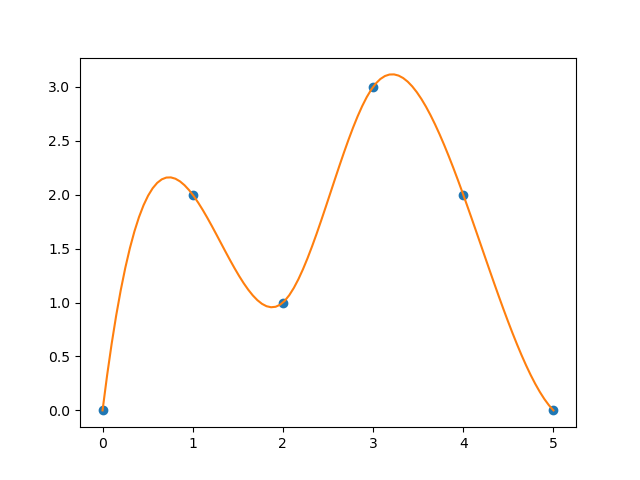
\includegraphics[width=1\linewidth]{Chapter2/graph/python/Figure2-5.png}
    \caption{自然边界条件的三次样条插值}
    \label{fig:自然边界条件三次样条插值}
\end{figure}

若想采用其他边界条件, 如希望采用固支边界条件, 并令端点一阶导数为0, 则可以在Python当中使用如下代码:

\begin{lstlisting}
# 三次样条插值演示(固支边界条件) Exercise2-7.py

import numpy as np
from scipy.interpolate import CubicSpline
import matplotlib.pyplot as plt

# 创建一些数据点
x = np.array([0, 1, 2, 3, 4, 5])
y = np.array([0, 2, 1, 3, 2, 0])

# 使用CubicSpline函数进行样条插值, 且端点一阶导数值为0
cs = CubicSpline(x, y, bc_type=((1,0),(1,0)))

# 生成插值点
x_interp = np.linspace(0, 5, 100)
y_interp = cs(x_interp)

# 绘制原始数据和插值曲线
plt.plot(x, y, 'o')
plt.plot(x_interp, y_interp)
plt.show()
\end{lstlisting}

所得图像如图\ref{fig:固支边界条件的三次样条插值}所示

\begin{figure}[h]
    \centering
    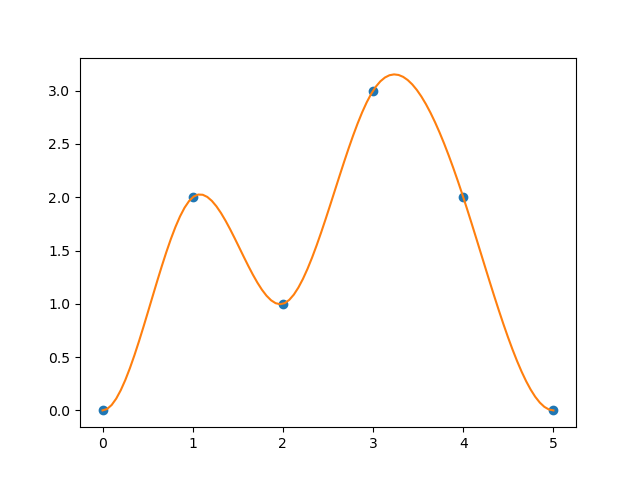
\includegraphics[width=1\linewidth]{Chapter2/graph/python/Figure2-6.png}
    \caption{固支边界条件的三次样条插值}
    \label{fig:固支边界条件的三次样条插值}
\end{figure}